\section{Grundlagen der GUI Programmierung}
Apps bestehen aus lose gekoppelten, wiederverwendbaren Komponenten. Diese sind Activities (für den Benutzer sichtbar) und Services, Content Provider, Broadcast Receivers (unsichtbar für Benutzer). Das System hat die Kontrolle über alle Applikationen und Verwaltet den Lebenszyklus, ist verantwortlich für die Kommunikation zwischen Komponenten und schliesst die Apps automatisch um Speicher zu sparen.
\paragraph{Activites} Dies sind die Hauptbausteine in der App Entwicklung, die Activity interagiert mit dem Benutzer.
\begin{lstlisting}
public class MainActivity extends Activity {
    @Override
    protected void onCreate(Bundle savedInstanceState) {
        super.onCreate(savedInstanceState);
        /* ... */
    }
}
\end{lstlisting}
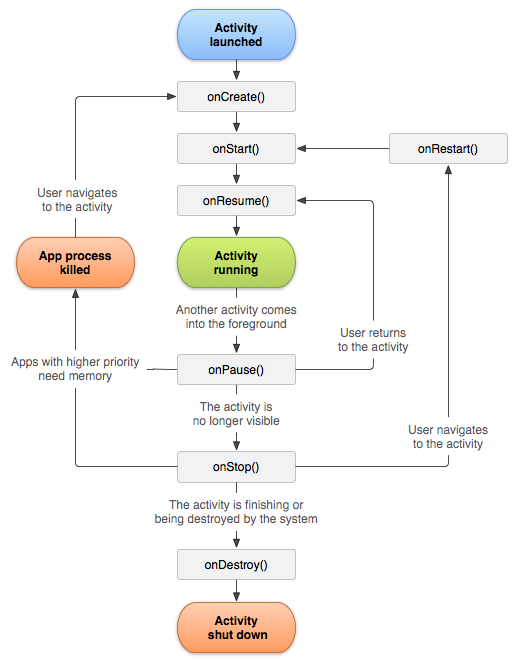
\includegraphics[scale=0.35]{activity_lifecycle.png}
Activities werden in einem Stack verwaltet, wobei die Activites eines Stacks zu verschiedenen Apps gehören können.\\
Eine Gruppe von Activities in einem Stack nennt man auch \textbf{Task}. Es können mehrere Tasks gleichzeitig existieren. 
\paragraph{Activity Launch Modes} Activities haben verschiedene Launch Modes
\begin{itemize}
\item \textbf{Standard:} Es wird eine neue Activity in den Stack gepusht
\item \textbf{SingleTop:} Ist Activity A zuoberst auf dem Stack und sie wird nochmals gestartet, wird in Activity A \code{onNewIntent()} ausgeführt
\item \textbf{SingleTask:} Das System erstellt einen neuen Task und instanziert die Activity als die Root des neuen Tasks. Wenn aber schon eine Instanz dieser Activity existiert, wird \code{onNewIntent()} in dieser aufgerufen. 
\item \textbf{SingleInstance:} Es darf nur eine Instanz der Activity geben
\end{itemize}
\paragraph{Intent} Ein Intent beschreibt was gemacht werden soll und das System entscheidet wer zuständig ist. Apps können selbst wiederum Activites zur Verfügung stellen und bestehende Applikationen ersetzen. Andere Activities können explizit oder implizit aufgerufen werden:
\begin{lstlisting}
// Explizit mit Klasse
Intent in = new Intent(this, CalculateActivity.class)
// Implizit mit Aktion
Intent in = new Intent(MediaStore.ACTION_IMAGE_CAPUTRE)
\end{lstlisting}
Andere Activities kann man mit \code{startActivity(intent)} oder \code{startActivityForResult(intent, myId)} starten. Um bei letzterem mit dem Rückgabewert arbeiten zu können muss man \code{onActivityResult} überschreiben.
\begin{lstlisting}
@Override
protected void onActivityResult(int request, int result, Intent data) {
    if (result == Activity.RESULT_OK && request == myId) {
        /* ... */
    }
}
\end{lstlisting}
Möchte man einem Intent Daten übergeben, kann man das entweder mit der \code{setData} Methode, welche eine URI entgegennimmt, oder mit \code{putExtra(MediaStore.EXTRA\_OUTPUT, imageCaptureUri)}. Letzere ist eine Struktur mit Key-Value Paaren und nimmt nur primitive Daten, Strings und serialisierbare Datentypen an.
\paragraph{Manifest} Das Manifest enthält Meta-Daten einer App. Es umfasst
\begin{itemize}
\item Komponenten der App
\item Metadaten (Name, Icon, Versionsnummer)
\item Permissions (Internet, kostenpflichtige Anrufe etc.)
\item Anforderungen an die Geräte API
\end{itemize}
Das Manifest wird vom System verwendet um zu wissen, ob die App installiert werden kann, welche Permissions diese verwendet etc.
\subsection{Android GUI}
\paragraph{Aufbau} Die Basisklasse um User Interfaces zu bauen ist die \code{View}. Eine View ist zuständig seinen Inhalt zu zeichnen und Events zu behandeln. Untergruppen der View sind Widgets und ViewGroups. Widgets ist ein Sammelbegriff für alle fix-fertigen Komponenten für User-Interfaces (Buttons, Images, Checkboxes etc.)
\paragraph{ViewGroup} Die ViewGroup ist eine Unterklasse von View. Sie kann andere View beinhalten. Wenn die ViewGroup beinhaltende View anordnet, spricht man von einem Layout.
\paragraph{Basis Layout} Layouts sind ViewGroups und beschreiben die visuelle Struktur des UIs.
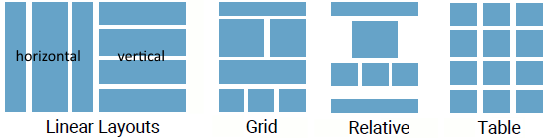
\includegraphics[scale=0.45]{layouts.png}
Die Layout-Parameter beschreiben wie die Views angeordnet und dargestellt werden. Für alle ViewGroups gemeinsam sind \code{android:layout\_width} und \code{android:layout\_height}. Häufig benutze Werte sind \code{match\_parent} (So gross wie mögich, also wie der Parent erlaubt) und \code{wrap\_content} (so klein wie möglich, also wie die Kinder erlauben).\\
In einem \textbf{Linear Layout} werden die Elemente horizontal oder vertikal angeordnet. Mit \code{android:layout\_weight} kann man Elementen ein Gewicht geben, da es selten sinnvoll ist, alle Elemente gleich gross zu lassen. Kinder ohne Weight bekommen minimalen Platz, auf die restlichen wird der verfügbare Platz nach Gewicht aufgeteilt.\\
Das \textbf{Relative Layout} ist das vielseitigse Layout welches Kinder relative zueinander anordnet.
\begin{lstlisting}[language=xml]
<RelativeLayout xmlns:android="... >
    <TextView
        android:text="1. Platz"
        android:id=@+id/first"
        android:layout_centerHorizontal="true" />
    <TextView
        android:text="2. Platz"
        android:id="@+id/first"
        android:layout_below="@id/first"
        android:layout_toStartOf="@id/first" />
    <TextView
        android:text="3. Platz"
        android:id="@+id/textView3"
        android:layout_below="@id/first"
        android:layout_toEnfOf="@id/first" />
</RelativeLayout>
\end{lstlisting}
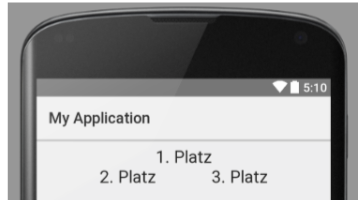
\includegraphics[scale=0.25]{RelativLayout.png} \\
Das \textbf{Frame Layout} kann die Kinder übereinander anordnen (Hilfslinien bei einer Kamera-App).\\
Das Layout muss in der Activity deklariert werden. Dies wird in der Activit Klasse mit \code{setContentView(R.layout.activity\_main)} gemacht.\\
\subsection{Widgets}
\paragraph{Button} Vom Button gibt es einen normalen \code{Button} und einen \code{ImageButton} bei dem man mit dem \code{android:src} ein Bild einfügen kann.
\paragraph{Eingabefelder} Der Typ des Eingabefeld bestimmt welche Tastatur verwendet wird. Dies kann man mit dem \code{android:inputType} bestimmen, es sind auch Kombinationen möglich. Innerhalb \code{EditText}
\paragraph{Referenzen und ID} Möchte man GUI-Elemente referenzieren, gibt man ihnen einen ID-String, welche Strings sind, die mit \code{@} beginnen. Wenn man einen neue ID definieren will, macht man das mit \code{@+id/}. Das Android-Buildsystem sammelt alle diese IDs als Konstanten in der automatisch generierten Klasse R. Diese Klasse enthält alle Ressourcen als Konstanten. Weitere Resourcesn sind: \code{drawable} (Bilder), \code{menu} (Menüs), \code{mipmap} (Launcher Icon der App) und \code{values} (Strings und andere Konstanten). Mit Aussnahme der values, wird für jeden Ordner eine innere Klasse in R generiert.
\paragraph{Dimensionen in Ressourcen} Konstanten in \code{dimens.xml} werden für Grössen in den Layouts benutzt.
\begin{lstlisting}[language=xml]
<!-- Layout -->
<RelativeLayout xmlns:android="..." xmlns:tools="..."
    android:layout_width="match_parent"
    android:layout_height="match_parent"
    android:paddingLeft="@dimen/activity_horizontal_margin"
    android:paddingRight="@dimen/activity_horizontal_margin"
    android:paddingTop="@dimen/activity_vertical_margin"
    android:paddingBottom="@dimen/activity_vertical_margin"
    tools:context=".MainActivity">
<!-- dimens.xml -->
    <!-- Default screen margins, per the Android Design guidelines. -->
    <dimen name="activity_horizontal_margin">16dp</dimen>
    <dimen name="activity_vertical_margin">16dp</dimen>
</resources>
\end{lstlisting}
Grössenangeben von Views erfolgen in density-indepentent Pixels (dp oder dip). Bei Schriften verwendet man scale-independent Pixels (sp).
\paragraph{Events und Event Handling}\label{grundlagen:eventhandling} Das Android-Framework hat einen sogenannten Event-Loop (Looper). Dieser wartet bis ein Ereignis passiert und verarbeitet dieses dann. Nur der Main-Thread darf das GUI verändern. \\
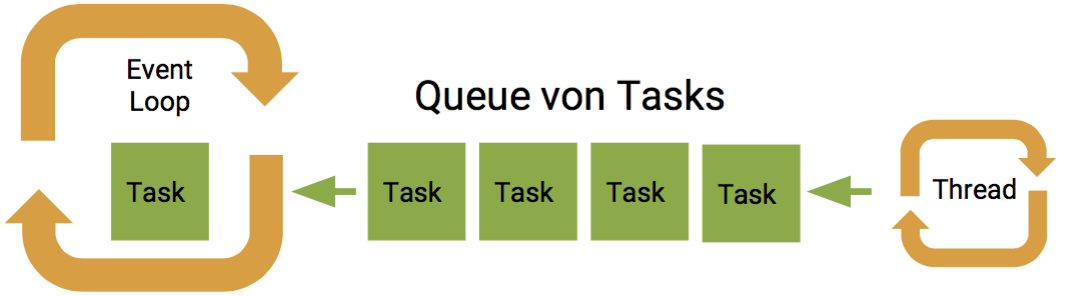
\includegraphics[scale=0.25]{EventLoops.png} \\
Fast alle Listener können mit \code{set[EventName]Listener} registriert werden.
\begin{lstlisting}
button.setOnClickListener(new View.OnClickListener() {
    @Override
    public void onClick(View v) {
        /* ... */
    }
});
\end{lstlisting}
Oder onClick Listener in XML deklariert
\begin{lstlisting}[language=xml]
android:onClick="onButtonClicked"
\end{lstlisting}
Alternativ zur anonymen Klasse, kann die Activity auch das Interface implementieren.
Bei der Verarbeitung von Texteingaben haben wir mehrere Möglichkeiten auf Events zu reagieren. Das zu implementierene Interface (\code{TextWatcher}) umfasst 3 Methoden:
\begin{itemize}
\item \code{beforeTextChanged}: Wird aufgerufen bevor der Text geändert wird
\item \code{onTextChanged}: Wird aufgerufen sobald der Text geändert hat
\item \code{afterTextChanged}: Nachdem der Text geändert wurde, kann man den Text noch anpassen (Loop-Gefahr)
\end{itemize}
\begin{lstlisting}
editText.addTextChangedListener(new TextWatcher() {
    public void onTextChanged(CharSequence s, int start, int before, int count){ }
    public void beforeTextChanged(CharSequence s, int start, int count, int after){ }
    public void afterTextChanged(Editable s) { }
});
\end{lstlisting}
Bei Eingabefeldern kann man mit \code{setError} Meldungen anzeigen lassen. Dies eignet sich gut für eine Inputvalidierung. Bei jeder Änderung wird diese zurückgesetzt.
\begin{lstlisting}
final EditText password = (EditText) findViewById(R.id.password);
password.addTextChangedListener(new TextWatcher() {
    @Override
    public void afterTextChanged(Editable s) {
        String pw = s.toString();
        if (s.length() < 8) {
        password.setError("Passwort muss mindestens 8 Zeichen lang sein.");
        }
    }
    ...
});
\end{lstlisting}
\subsection{Android Testing mit JUnit}
Es gibt mehrere Arten von Tests für eine Activity. Die \code{ActivityUnitTest} manipulieren das UI im Code, die \code{ActivityInstrumentationTestCase2} schickt Clicks und Events an das UI. Um eine App mit mehreren Activities zu testen, gibt es das Espresso Framework, sowie UI Automator um App-übergreifend zu testen.
\begin{lstlisting}
public class MainActivityLayoutTest extends ActivityUnitTestCase<MainActivity> {
    public MainActivityLayoutTest() {
        super(MainActivity.class);
    }
    @Override
    protected void setUp() throws Exception {
        super.setUp();
        ContextThemeWrapper context = new
            ContextThemeWrapper(getInstrumentation().getTargetContext(), R.style.AppTheme);
        setActivityContext(context);
        startActivity(
            new Intent(getInstrumentation().getTargetContext(), MainActivity.class),null,null);
}
\end{lstlisting}
Funktionale Tests (ActivityInstrumentationTestCase2) testen eine Activity im echten Systemkontext. Der Test löst Events aus und prüft, ob diese zum erwünschten Resultat führen. Dazu gehören: 
\begin{itemize}
\item Ändert sich das UI wie erwartet
\item Überprüfen von Inputvalidierung
\item Werden Lifecycle Events korrekt behandelt
\end{itemize}
\begin{lstlisting}
public class MainActivityInteractionTest extends ActivityInstrumentationTestCase2<MainActivity> {
    public MainActivityInteractionTest() { super(MainActivity.class); }
    public void testSayHi() {
        MainActivity activity = getActivity();
        final EditText editText = (EditText) activity.findViewById(R.id.editText);
        getInstrumentation().runOnMainSync(new Runnable() {
            @Override
            public void run() {
                editText.requestFocus();
            }
        });
        getInstrumentation().waitForIdleSync();
        getInstrumentation().sendStringSync("Hello");
        getInstrumentation().waitForIdleSync();
        Button button = (Button) activity.findViewById(R.id.button);
        TouchUtils.clickView(this, button);
...
\end{lstlisting}
